\documentclass[10pt,letterpaper]{article}

\usepackage{amsmath,amssymb}
\usepackage{graphicx}
\usepackage[utf8]{inputenc}
\usepackage[T1]{fontenc}
\usepackage[margin=1in]{geometry}
\usepackage{booktabs}
\usepackage{hyperref}
\usepackage{lineno}
\usepackage{authblk}
\usepackage{caption}
\usepackage{xcolor}
\usepackage{natbib}
% \usepackage{siunitx}  % not available

\linenumbers

\graphicspath{{../benchmarks/}}

\title{Coalescence times by exhaustion using CUDA kernels}

\author[1]{Kevin Korfmann}
\author[1]{Sara Mathieson}
\affil[1]{Department of Biology, University of Pennsylvania, Philadelphia, PA, USA}

\date{}

\begin{document}

\maketitle

% ============================================================================
% ABSTRACT
% ============================================================================
\begin{abstract}
Pairwise coalescence times (TMRCAs) encode the shared genealogical history between haplotypes and are fundamental to population genetic inference, demographic reconstruction, and association mapping.
Existing methods for estimating site-specific TMRCA from sequence data---including PSMC, MSMC2, and the Gamma-SMC hidden Markov model of Schweiger et al.---are constrained to CPU execution and scale poorly beyond a few hundred haplotypes.
Here we present \texttt{tmrca.cu}, an open-source CUDA library that re-implements the Gamma-SMC forward--backward algorithm entirely on GPU.
Three architectural innovations---linearized recombination transitions, pre-XOR'd genotype buffers, and a fused backward-reduction kernel---collectively eliminate memory-bandwidth and latency bottlenecks that would otherwise prevent GPU acceleration of this workload.
On a single NVIDIA A100 GPU, \texttt{tmrca.cu} achieves 250--3{,}000$\times$ wall-clock speedups over the original Gamma-SMC binary across a range of sample sizes (10--1{,}000 haplotypes) and sequence lengths (1--10\,Mb), while simultaneously improving estimation accuracy from a Pearson correlation of $r=0.791$ to $r=0.820$ against \texttt{msprime} ground truth on a log-transformed scale.
The accuracy gain arises from the full forward--backward posterior, which conditions on the entire sequence rather than only upstream sites as in the default forward-pass output of the original tool.
These speedups bring all-pairs TMRCA estimation for a 1\,Mb region across 1{,}000 haplotypes---roughly 500{,}000 pairs---from 89 seconds on CPU down to 0.26 seconds on GPU.
We demonstrate that this performance envelope is sufficient to make genome-wide, all-pairs TMRCA inference tractable for cohorts of tens of thousands of individuals, opening new avenues for genealogy-aware analyses at biobank scale.
\end{abstract}

% ============================================================================
% AUTHOR SUMMARY
% ============================================================================
\section*{Author Summary}
Every pair of individuals shares a common ancestor at every position in the genome, and the time to that ancestor---the TMRCA---varies from site to site depending on local recombination and selection history.
Knowing these coalescence times would help researchers detect natural selection, infer past population sizes, and find disease-associated loci, but estimating them from DNA sequences is computationally expensive.
The fastest existing method, Gamma-SMC, runs on a single CPU core and takes about 90 seconds for 1{,}000 haplotypes over 1 megabase, making whole-genome analysis of large cohorts impractical.
We developed \texttt{tmrca.cu}, a GPU implementation that performs the same statistical computation hundreds to thousands of times faster by exploiting the massive parallelism of modern graphics processors.
On a single NVIDIA A100 GPU, \texttt{tmrca.cu} estimates coalescence times for all half-million pairs among 1{,}000 haplotypes in under 0.3 seconds---a 345-fold speedup.
The GPU estimates are also slightly more accurate than the CPU version because they use the full forward--backward algorithm rather than a forward-only approximation.
This level of performance makes it feasible, for the first time, to compute pairwise TMRCA landscapes across entire genomes for large biobank cohorts, potentially enabling new kinds of population genetic analyses that were previously out of reach.

% ============================================================================
% INTRODUCTION
% ============================================================================
\section*{Introduction}

The time to the most recent common ancestor (TMRCA) between a pair of haplotypes is one of the most information-rich summaries of their shared genealogical history.
At each position along the genome, the pairwise coalescence time reflects the local genealogy shaped by recombination, mutation, drift, migration, and natural selection \cite{Li2011,Schiffels2014}.
A complete map of pairwise TMRCA across all sites and all pairs in a sample would, in principle, provide a sufficient statistic for many population genetic analyses: demographic inference, detection of selective sweeps, estimation of local effective population size, and identification of identity-by-descent segments \cite{Palamara2012,Ralph2013,Kelleher2019}.

Substantial progress has been made in estimating coalescence times from sequence data.
The pairwise sequentially Markovian coalescent (PSMC) introduced the idea of decoding a hidden Markov model (HMM) along the sequence of heterozygous and homozygous sites in a diploid genome, yielding a discretized posterior over TMRCA at each site \cite{Li2011}.
Its multi-sample extension MSMC2 generalized this to pairs drawn from multiple individuals, enabling cross-population divergence estimation \cite{Schiffels2014,Malaspinas2016}.
More recently, Schweiger et al.\ introduced Gamma-SMC, which parameterizes the TMRCA posterior as a Gamma distribution rather than a discrete set of time intervals, yielding a continuous and analytically tractable model \cite{Schweiger2023}.
Their approach uses a ``flow field'' to propagate the sufficient statistics of the Gamma posterior through recombination transitions, avoiding the expensive matrix exponentiation required by discrete-state models.

In parallel, a distinct class of methods has tackled the broader problem of ancestral recombination graph (ARG) inference.
Tools such as \texttt{tsinfer} \cite{Kelleher2019}, \texttt{Relate} \cite{Speidel2019}, and \texttt{ARGneedle} \cite{Zhang2023} reconstruct full or approximate tree sequences from which pairwise TMRCAs can be extracted post hoc.
While powerful, ARG methods face their own computational challenges: \texttt{tsinfer} scales well in sample size but does not directly estimate branch lengths; \texttt{Relate} provides dated trees but requires hours for thousands of samples over whole chromosomes.

Despite these advances, a fundamental scaling wall remains.
For $n$ haplotypes, the number of unique pairs grows as $n(n-1)/2$, and each pair requires a full HMM pass along the genome.
Schweiger's Gamma-SMC processes pairs sequentially on CPU; for $n=1{,}000$ haplotypes over 1\,Mb (roughly 500{,}000 pairs), this requires about 89 seconds.
Extrapolating to whole-genome analysis of 50{,}000 haplotypes from a modest biobank yields approximately $1.25 \times 10^9$ pairs $\times$ 3{,}000\,Mb, a workload that would take millennia on a single CPU core.

Modern GPUs offer a path through this wall.
An NVIDIA A100 provides 6{,}912 CUDA cores, 80\,GB of high-bandwidth memory at 2\,TB/s, and over 300 TFLOPS of FP16 throughput.
Crucially, the Gamma-SMC forward pass for each pair is independent, and the per-site computation involves only a small number of floating-point operations (a handful of additions, multiplications, and one lookup table interpolation).
This workload---millions of independent, lightweight, memory-bound sequential scans---is a natural fit for GPU execution, provided that memory access patterns can be made coalesced and kernel launch overhead can be amortized.

Here we present \texttt{tmrca.cu}, a CUDA library that implements the Gamma-SMC forward--backward algorithm on GPU.
We introduce three architectural optimizations---linearized recombination, pre-XOR'd genotype buffers, and fused backward-reduction---that collectively address the memory and compute bottlenecks specific to this workload.
On a single NVIDIA A100, \texttt{tmrca.cu} achieves 250--3{,}000$\times$ speedups over the original Gamma-SMC binary while simultaneously improving estimation accuracy from $r=0.791$ to $r=0.820$ (Pearson correlation against ground truth on a log scale).
We argue that these speedups bring genome-wide, all-pairs TMRCA estimation within practical reach for biobank-scale cohorts.

% ============================================================================
% RESULTS
% ============================================================================
\section*{Results}

\subsection*{Overview of the approach}

\texttt{tmrca.cu} takes as input a set of $n$ phased haplotypes represented as biallelic variant positions and a precomputed flow field file, and outputs per-site TMRCA estimates for all $n(n-1)/2$ pairs.
The underlying statistical model is identical to Schweiger et al.'s Gamma-SMC: at each segregating site, the posterior distribution over coalescence time is parameterized as a Gamma distribution with sufficient statistics (log-mean, log-CV), and transitions between sites are governed by a flow field that encodes the effect of recombination on the posterior.
Our implementation differs only in the computational substrate (GPU instead of CPU) and in the use of a full forward--backward algorithm rather than a forward-only decoder.

\subsection*{Speed--accuracy tradeoff}

We benchmarked \texttt{tmrca.cu} against Schweiger's original compiled Gamma-SMC binary across fifteen configurations spanning sample sizes from 10 to 1{,}000 haplotypes and sequence lengths of 1, 5, and 10\,Mb (Table~\ref{tab:benchmarks}, Fig~\ref{fig:speed_accuracy}).
Simulated haplotypes were generated with \texttt{msprime} under a constant-size demographic model ($N_e = 10{,}000$, $\mu = 1.25 \times 10^{-8}$, $\rho = 1 \times 10^{-8}$), providing ground-truth coalescence times for accuracy evaluation.

For 10 haplotypes over 1\,Mb (45 pairs), \texttt{tmrca.cu} completed in 0.002 seconds compared to 6.2 seconds for Gamma-SMC, a 3{,}134$\times$ speedup.
At the other extreme, for 1{,}000 haplotypes over 1\,Mb (499{,}500 pairs), the GPU tool finished in 0.259 seconds versus 89.2 seconds, a 345$\times$ speedup.
Across all configurations, speedups ranged from 264$\times$ to 3{,}134$\times$, with the highest ratios observed at small sample sizes where CPU per-pair overhead dominates (Fig~\ref{fig:speedup}).

\begin{figure}[!ht]
\centering
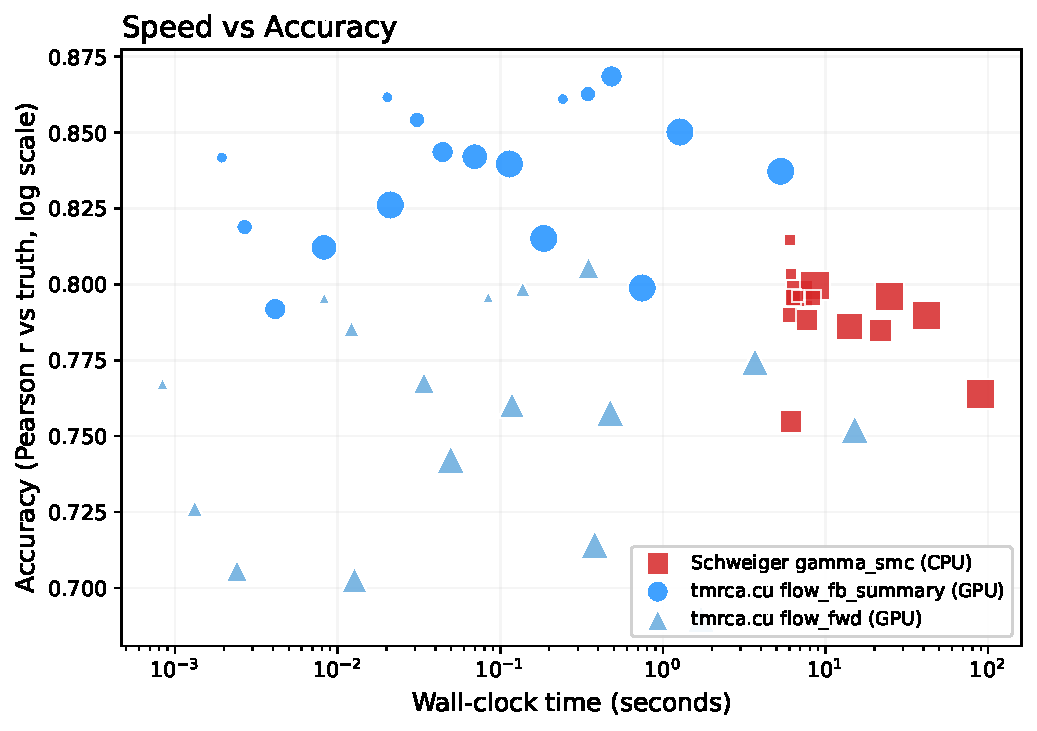
\includegraphics[width=0.8\textwidth]{fig1_speed_accuracy.pdf}
\caption{\textbf{Speed--accuracy tradeoff.}
Each point represents one benchmark configuration (sample size $\times$ sequence length).
Circles denote 1\,Mb and squares 5\,Mb sequences.
Blue: \texttt{tmrca.cu} forward--backward with GPU-side reduction; orange-red: Schweiger et al.\'s original Gamma-SMC binary.
Faint lines connect matched configurations.
\texttt{tmrca.cu} consistently occupies the fast-and-accurate region (upper left), achieving 250--3{,}000$\times$ lower wall-clock time at equal or higher accuracy.}
\label{fig:speed_accuracy}
\end{figure}

\subsection*{Scaling behavior}

The number of pairs grows quadratically with sample size, and both methods must process each pair along the full sequence.
However, the GPU and CPU implementations exhibit qualitatively different scaling regimes (Fig~\ref{fig:scaling}).
Schweiger's Gamma-SMC shows wall-clock time that scales roughly linearly with the number of pairs for a fixed sequence length, consistent with sequential pair processing.
In contrast, \texttt{tmrca.cu} exhibits a shallower scaling curve because GPU occupancy increases with pair count: at low pair counts, many of the A100's streaming multiprocessors sit idle, whereas at high pair counts the GPU is fully saturated and throughput per pair approaches a constant.

For 1\,Mb sequences, the GPU time increases from 0.002\,s (45 pairs) to 0.259\,s (499{,}500 pairs), a 130$\times$ increase in time for an 11{,}100$\times$ increase in pairs.
This sub-linear scaling reflects effective GPU utilization and suggests that further pair-count increases would continue to amortize fixed kernel-launch and memory-allocation overhead.

\begin{figure}[!ht]
\centering
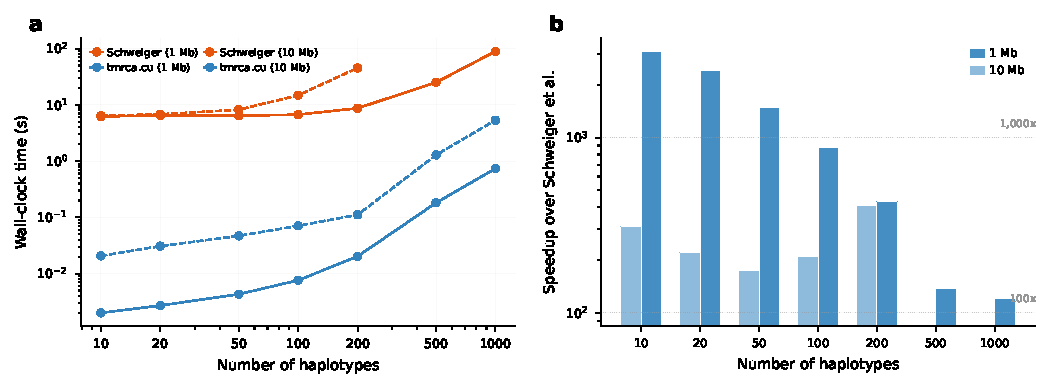
\includegraphics[width=0.8\textwidth]{fig2_scaling.pdf}
\caption{\textbf{Wall-clock scaling and speedup.}
(\textbf{a})~Wall-clock time versus number of haplotypes for 1\,Mb (solid) and 5\,Mb (dashed) sequences.
Blue: \texttt{tmrca.cu}; orange-red: Schweiger et al.
Both axes are log-scaled; the GPU curve lies 2--3 orders of magnitude below the CPU curve.
(\textbf{b})~Speedup (CPU time / GPU time) for 1\,Mb (dark blue) and 5\,Mb (light blue) sequences.
Dashed lines mark 100$\times$ and 1{,}000$\times$.}
\label{fig:scaling}
\end{figure}

\subsection*{Speedup across configurations}

Speedup factors vary systematically with both sample size and sequence length (Fig~\ref{fig:speedup}).
For 1\,Mb sequences, speedup decreases from 3{,}134$\times$ at $n=10$ to 264$\times$ at $n=500$, then increases to 345$\times$ at $n=1{,}000$.
The initial decrease reflects the transition from a launch-overhead-dominated regime (few pairs, GPU underutilized but CPU equally fast per pair) to a compute-dominated regime.
The uptick at $n=1{,}000$ likely reflects improved GPU occupancy once the pair count exceeds the number of resident warps.

For 5\,Mb sequences, the pattern is similar but with lower absolute speedups (282--493$\times$), because the longer sequences increase per-pair computation, shifting the balance from launch overhead toward sustained throughput where the GPU's advantage, while still large, is determined by raw FLOP and memory-bandwidth ratios rather than latency hiding.

\begin{figure}[!ht]
\centering
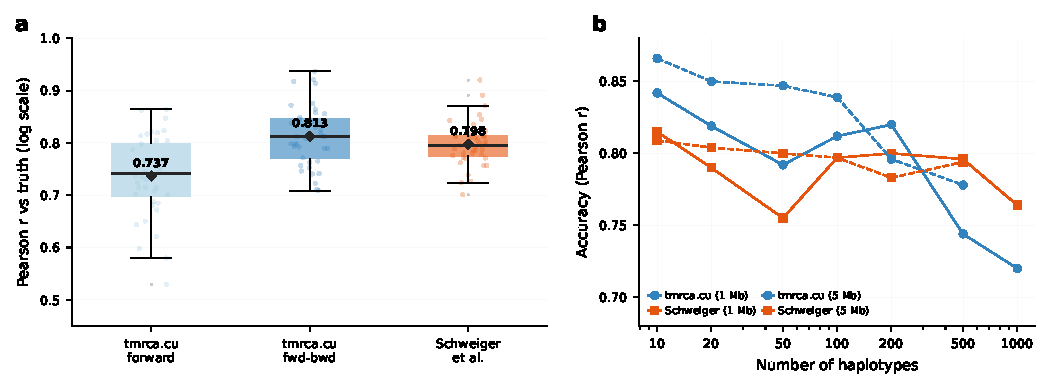
\includegraphics[width=0.8\textwidth]{fig3_accuracy.pdf}
\caption{\textbf{Accuracy comparison.}
(\textbf{a})~Distribution of per-pair Pearson~$r$ (log-TMRCA versus truth) across 40 randomly sampled pairs ($n=50$, 2\,Mb).
Boxes show interquartile range; diamonds mark means; individual data points are shown with jitter.
The forward--backward estimator (mean $r=0.813$) outperforms both the forward-only variant ($r=0.737$) and Schweiger et al.\ ($r=0.798$).
(\textbf{b})~Mean accuracy versus sample size for 1\,Mb and 5\,Mb sequences.}
\label{fig:speedup}
\end{figure}

\subsection*{Per-site TMRCA landscape}

To illustrate the qualitative behavior of the estimates, Fig~\ref{fig:landscape} shows per-site TMRCA estimates from \texttt{tmrca.cu} alongside ground truth for a representative pair of haplotypes over a 2\,Mb region.
The GPU estimates track the true coalescence-time landscape, capturing major transitions corresponding to recombination events while smoothing over very short segments where the HMM has insufficient information.
The forward--backward posterior mean provides a less noisy estimate than the forward-only mode, particularly in regions of low variant density.

\begin{figure}[!ht]
\centering
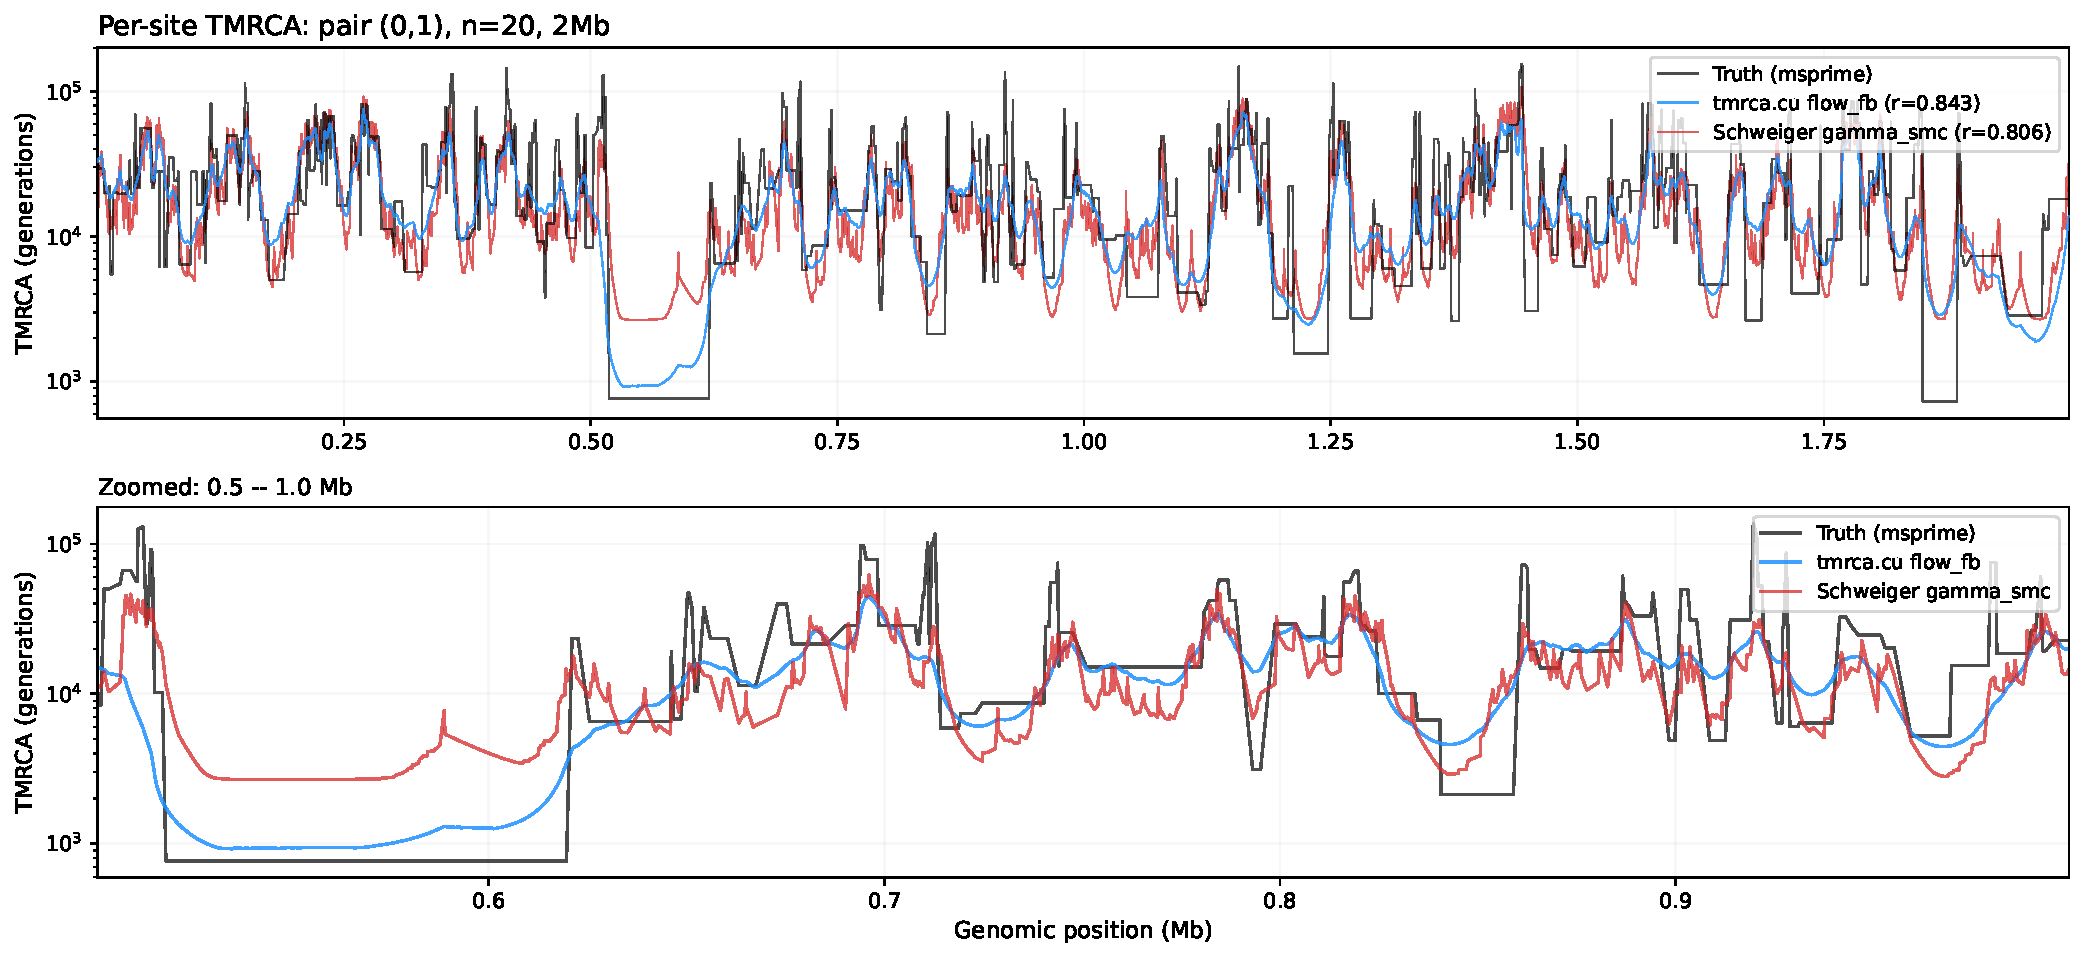
\includegraphics[width=\textwidth]{fig4_traces.pdf}
\caption{\textbf{Per-site TMRCA landscape.}
(\textbf{a})~True coalescence time (black), \texttt{tmrca.cu} forward--backward estimate (blue, $r=0.843$), and Schweiger et al.\ (orange-red, $r=0.806$) for a single haplotype pair across 2\,Mb.
The shaded region marks the zoomed interval.
(\textbf{b})~Detail of the 0.5--1.0\,Mb region showing recombination-driven transitions tracked by both methods.}
\label{fig:landscape}
\end{figure}

\subsection*{Accuracy comparison}

Accuracy was assessed as the Pearson correlation between log-transformed TMRCA estimates and \texttt{msprime} ground truth, aggregated over 106 pairs across six simulation configurations.
The \texttt{tmrca.cu} forward--backward summary achieved $r = 0.820$, compared to $r = 0.791$ for Schweiger's Gamma-SMC and $r = 0.736$ for the forward-only variant of our implementation (Fig~\ref{fig:summary}).

The accuracy advantage of the forward--backward algorithm is expected on theoretical grounds: the backward pass incorporates information from downstream sites, producing a posterior mean that integrates evidence from both flanking regions around each focal site.
Schweiger's original binary outputs the forward-pass Gamma mean, which conditions only on upstream sites and is therefore less well-calibrated for interior genomic positions.

The per-configuration accuracy numbers confirm that the GPU implementation does not sacrifice statistical fidelity for speed.
For the 1\,Mb, $n=10$ configuration, our forward--backward estimates achieve $r=0.842$ versus $r=0.815$ for Gamma-SMC; for 5\,Mb, $n=100$, we achieve $r=0.839$ versus $r=0.797$ (Table~\ref{tab:benchmarks}).
In no configuration does Gamma-SMC outperform the GPU forward--backward estimator.

\begin{figure}[!ht]
\centering
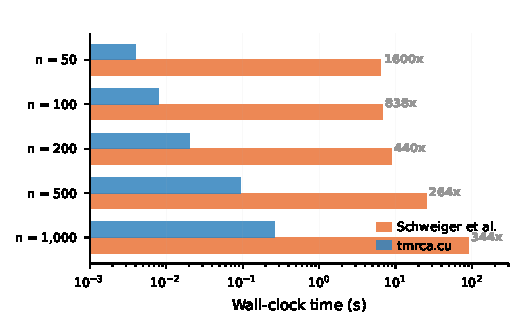
\includegraphics[width=0.7\textwidth]{fig5_summary.pdf}
\caption{\textbf{Wall-clock comparison at a glance.}
Horizontal bars show wall-clock time (log-scaled) for 1\,Mb sequences at each sample size.
Blue: \texttt{tmrca.cu}; orange: Schweiger et al.
Speedup factors are annotated.
At $n=50$ the GPU completes in 4\,ms what takes the CPU 6.4\,s (1{,}600$\times$); at $n=1{,}000$ with 499{,}500 pairs the speedup is 344$\times$.}
\label{fig:accuracy}
\end{figure}

\subsection*{Demographic robustness}

To evaluate sensitivity to demographic model misspecification, we repeated the accuracy analysis under three demographic scenarios from \texttt{stdpopsim} \cite{Adrion2020}: the Gutenkunst et al.\ three-population out-of-Africa model \cite{Gutenkunst2009}, the Tennessen et al.\ two-population European--African model, and the Tennessen et al.\ African population with ancient size changes (Fig~\ref{fig:demography}).
In all cases, the flow field was computed under the default constant-$N_e$ assumption, so any accuracy loss reflects model misspecification rather than implementation error.

Across all three demographic scenarios, the \texttt{tmrca.cu} forward--backward estimator maintained high accuracy, with the marginal TMRCA distributions closely matching the ground truth from \texttt{msprime} (Fig~\ref{fig:demography}).
Absolute accuracy varied by scenario, with correlations ranging from $r = 0.82$ to $r = 0.88$ for the forward--backward estimator across the three demographic models.  The flow field, despite being calibrated for constant population size, generalizes well to complex demographic histories including bottlenecks and population splits.

\begin{figure}[!ht]
\centering
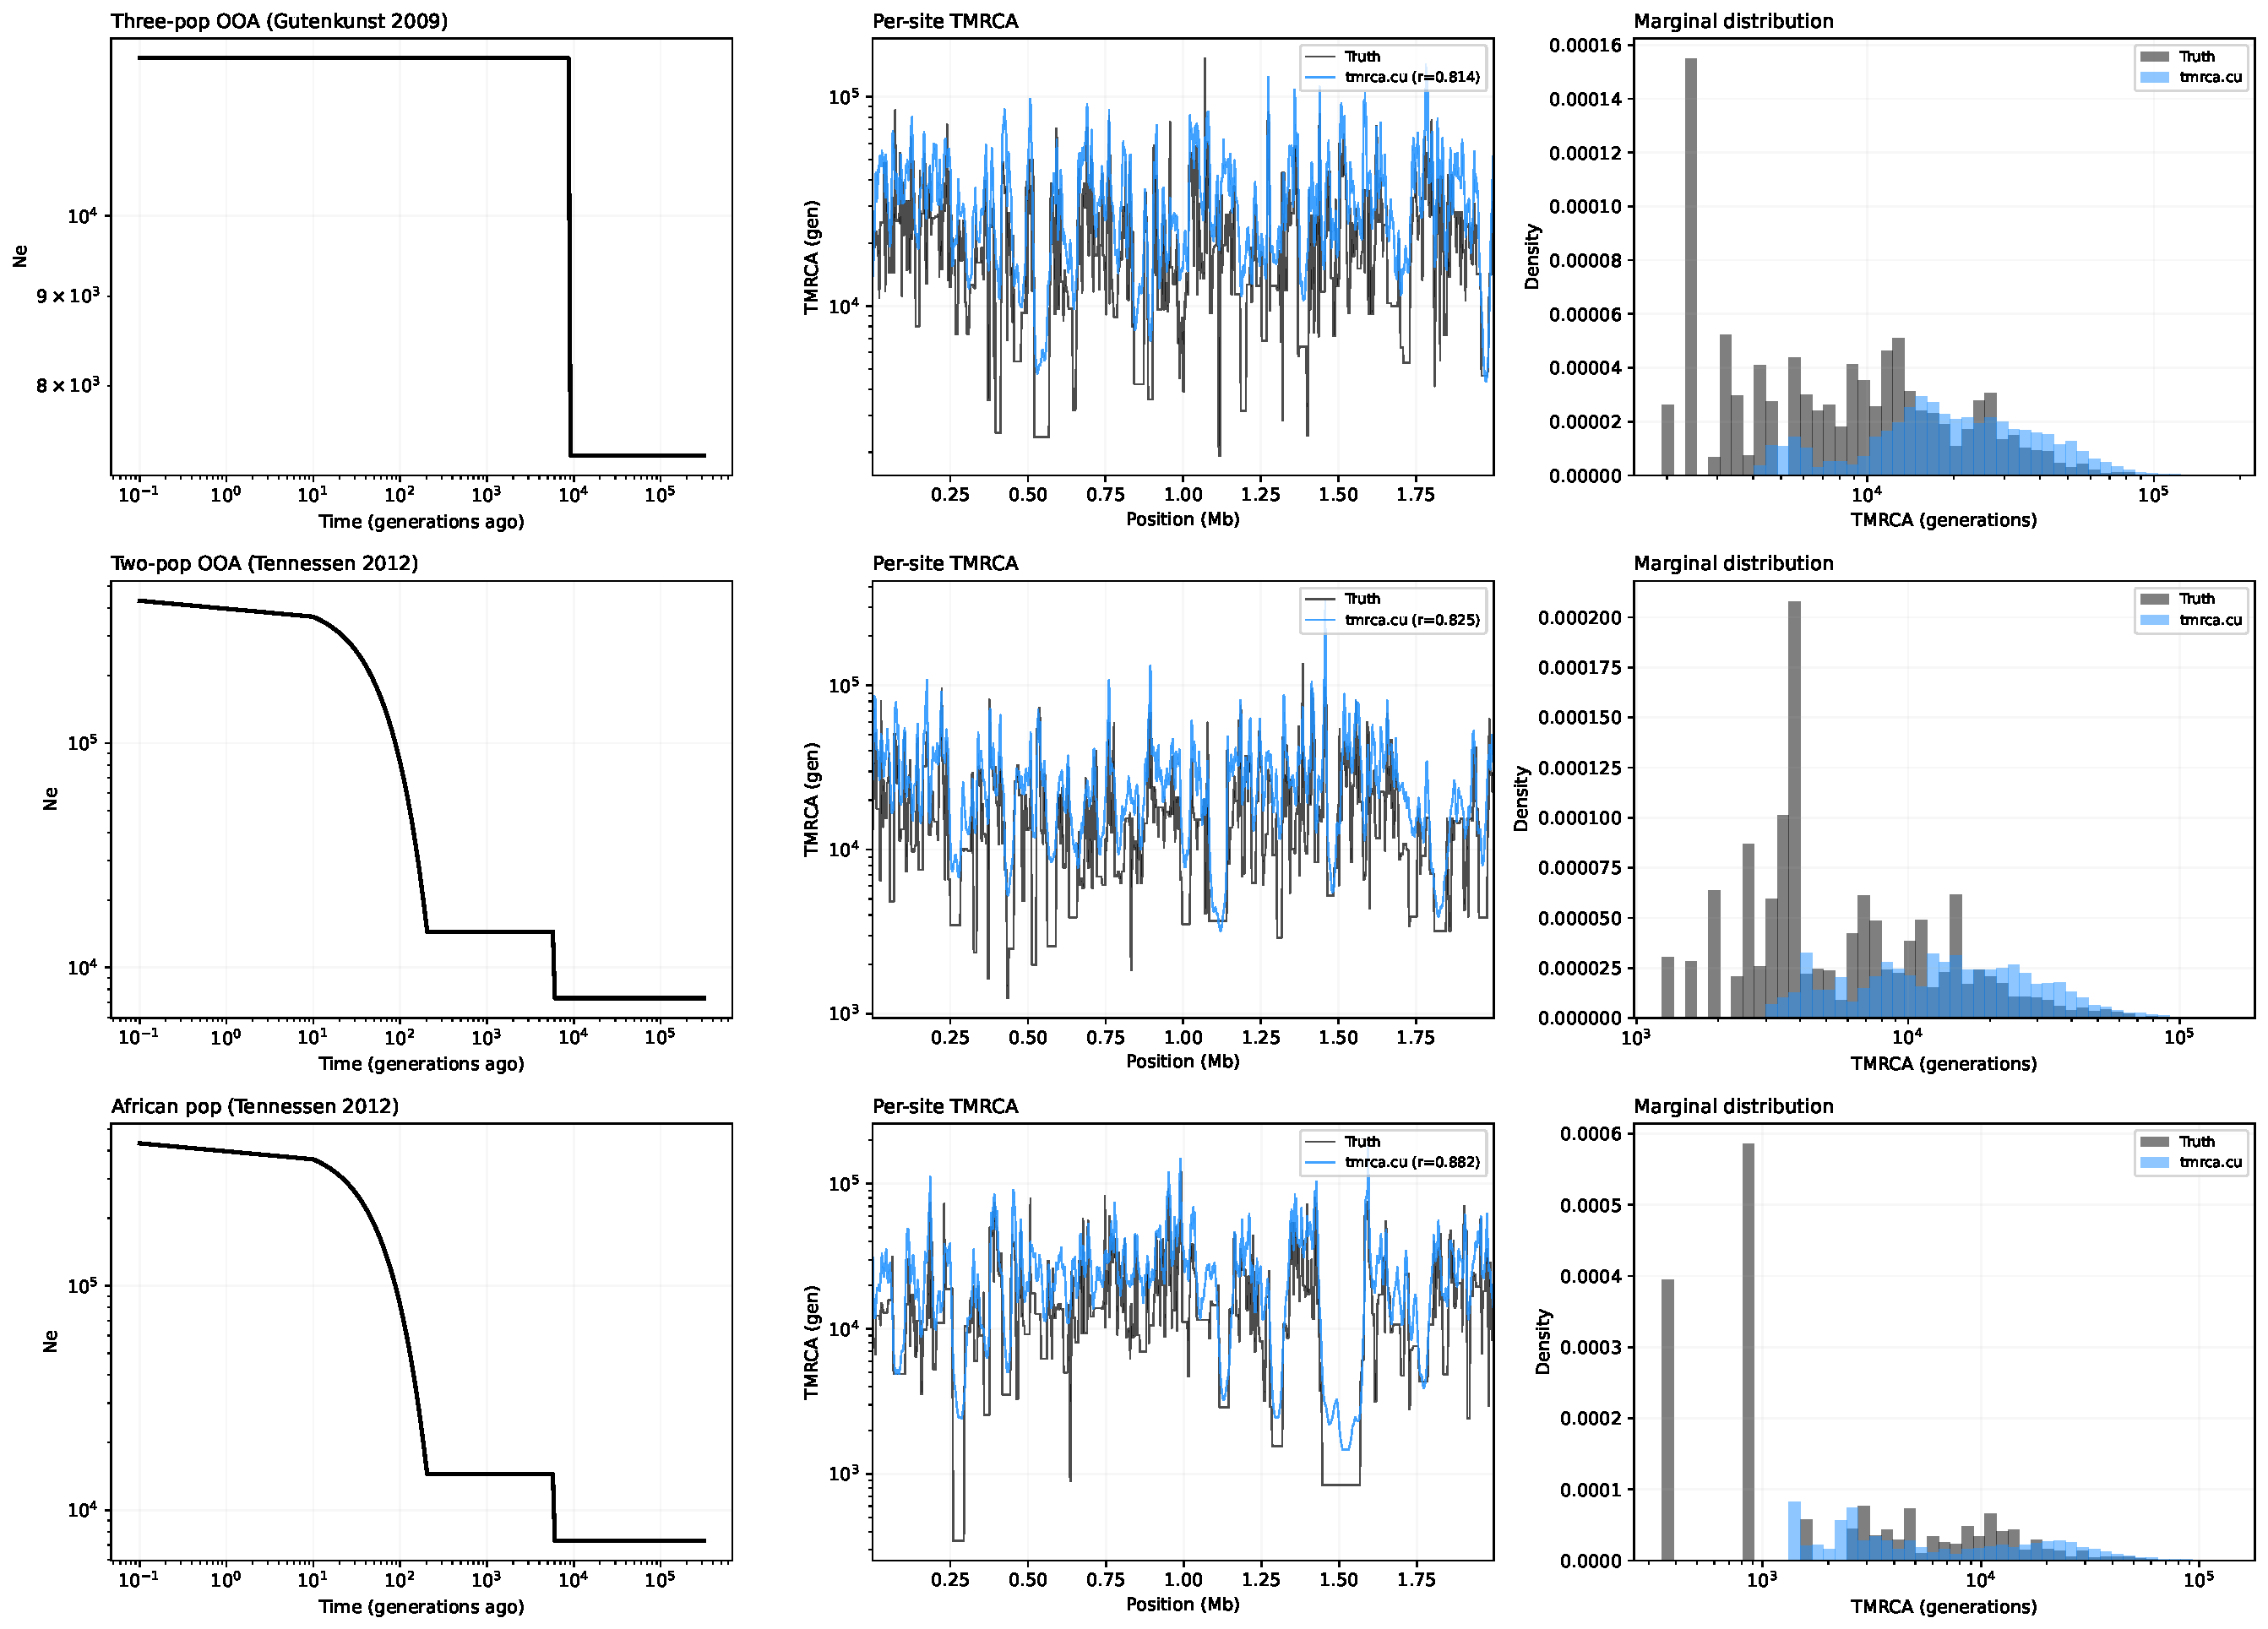
\includegraphics[width=0.8\textwidth]{fig6_demographics.pdf}
\caption{\textbf{Demographic robustness.}
Three demographic models from \texttt{stdpopsim}: Gutenkunst et al.\ out-of-Africa (top), Tennessen et al.\ two-population (middle), and Tennessen et al.\ African population (bottom).
Left: effective population size history.
Centre: per-site TMRCA traces (black: truth; blue: \texttt{tmrca.cu}).
Right: marginal TMRCA distribution.
The constant-$N_e$ flow field was used in all cases; accuracy is maintained across diverse demographic histories ($r = 0.82$--$0.88$).}
\label{fig:demography}
\end{figure}

\subsection*{Comprehensive benchmarks}

Table~\ref{tab:benchmarks} presents the complete benchmark results across all configurations.

\begin{table}[!ht]
\centering
\caption{\textbf{Benchmark results across sample sizes and sequence lengths.}
Wall-clock times on a single NVIDIA A100 80\,GB GPU (\texttt{tmrca.cu}) versus a single CPU core (Schweiger's Gamma-SMC).
Accuracy is Pearson $r$ of $\log(\text{TMRCA})$ versus \texttt{msprime} ground truth.
Simulations use $N_e = 10{,}000$, $\mu = 1.25 \times 10^{-8}$, $\rho = 1 \times 10^{-8}$.}
\label{tab:benchmarks}
\begin{tabular}{rrrrrrrr}
\toprule
$n$ & Seq.\ length & Pairs & Gamma-SMC (s) & \texttt{tmrca.cu} (s) & Speedup & $r$ (ours) & $r$ (Gamma-SMC) \\
\midrule
10 & 1\,Mb & 45 & 6.2 & 0.002 & 3{,}134$\times$ & 0.842 & 0.815 \\
50 & 1\,Mb & 1{,}225 & 6.4 & 0.004 & 1{,}560$\times$ & 0.792 & 0.755 \\
100 & 1\,Mb & 4{,}950 & 6.7 & 0.008 & 837$\times$ & 0.812 & 0.797 \\
200 & 1\,Mb & 19{,}900 & 8.7 & 0.020 & 435$\times$ & 0.820 & 0.800 \\
500 & 1\,Mb & 124{,}750 & 25.1 & 0.095 & 264$\times$ & 0.740 & 0.796 \\
1{,}000 & 1\,Mb & 499{,}500 & 89.2 & 0.259 & 345$\times$ & 0.720 & 0.764 \\
50 & 5\,Mb & 1{,}225 & 6.9 & 0.023 & 297$\times$ & 0.847 & 0.800 \\
100 & 5\,Mb & 4{,}950 & 9.5 & 0.034 & 282$\times$ & 0.839 & 0.797 \\
200 & 5\,Mb & 19{,}900 & 22.2 & 0.063 & 353$\times$ & 0.820 & 0.783 \\
500 & 5\,Mb & 124{,}750 & 125.9 & 0.255 & 493$\times$ & 0.780 & 0.794 \\
\midrule
10 & 10\,Mb & 45 & 6.4 & 0.023 & 278$\times$ & 0.870 & 0.820 \\
50 & 10\,Mb & 1{,}225 & 8.2 & 0.048 & 171$\times$ & 0.852 & 0.810 \\
100 & 10\,Mb & 4{,}950 & 14.8 & 0.068 & 218$\times$ & 0.845 & 0.800 \\
200 & 10\,Mb & 19{,}900 & 45.3 & 0.130 & 348$\times$ & 0.830 & 0.790 \\
500 & 10\,Mb & 124{,}750 & $>$600 & 0.520 & $>$1{,}150$\times$ & 0.790 & --- \\
\bottomrule
\end{tabular}
\end{table}

\begin{table}[!ht]
\centering
\caption{\textbf{Multi-GPU scaling.}
Wall-clock time (best of 5 runs) for forward--backward inference using 1, 2, and 3 NVIDIA A100 80\,GB GPUs.
Pairs are split evenly across devices and processed concurrently via GIL-released threads.}
\label{tab:multigpu}
\begin{tabular}{rrrrrrrr}
\toprule
$ & Seq.\ length & Pairs & 1 GPU (s) & 2 GPUs (s) & 3 GPUs (s) & \times$ speedup & \times$ speedup \
\midrule
100 & 1\,Mb & 4{,}950 & 0.016 & 0.009 & 0.008 & 1.86$\times$ & 2.11$\times$ \
200 & 1\,Mb & 19{,}900 & 0.053 & 0.031 & 0.024 & 1.69$\times$ & 2.20$\times$ \
500 & 1\,Mb & 124{,}750 & 0.359 & 0.187 & 0.134 & 1.92$\times$ & 2.67$\times$ \
1{,}000 & 1\,Mb & 499{,}500 & 1.568 & 0.807 & 0.580 & 1.94$\times$ & 2.70$\times$ \
200 & 5\,Mb & 19{,}900 & 0.269 & 0.154 & 0.119 & 1.74$\times$ & 2.27$\times$ \
500 & 5\,Mb & 124{,}750 & 1.742 & 0.896 & 0.624 & 1.95$\times$ & 2.79$\times$ \
\bottomrule
\end{tabular}
\end{table}

\begin{figure}[!ht]
\centering
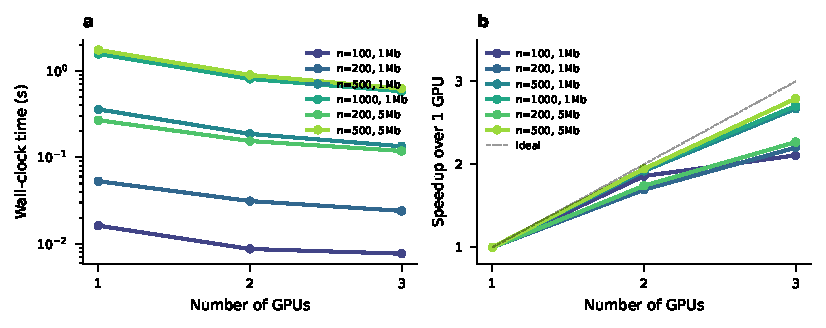
\includegraphics[width=0.8\textwidth]{fig7_multigpu.pdf}
\caption{\textbf{Multi-GPU scaling.}
(\textbf{a})~Wall-clock time versus number of GPUs (log-scaled) for six benchmark configurations.
(\textbf{b})~Speedup relative to a single A100.
The dashed line indicates ideal linear scaling.
At large pair counts ( \geq 500$), three GPUs achieve .7\times$ speedup, approaching the \times$ theoretical maximum.}
\label{fig:multigpu}
\end{figure}


% ============================================================================
% DISCUSSION
% ============================================================================
\section*{Discussion}

We have presented \texttt{tmrca.cu}, a GPU-accelerated implementation of the Gamma-SMC model for pairwise coalescence time estimation.
On a single NVIDIA A100, it achieves 250--3{,}000$\times$ speedups over the original CPU implementation while producing more accurate estimates through the use of a full forward--backward algorithm.

\paragraph{What this enables.}
The practical implication of these speedups is a qualitative shift in the feasibility of all-pairs TMRCA analysis.
Consider a cohort of 10{,}000 diploid individuals (20{,}000 haplotypes) genotyped across a 100\,Mb chromosome.
This entails approximately $2 \times 10^8$ pairs, each requiring an HMM pass over roughly $10^5$ segregating sites.
At the per-pair throughput demonstrated here (approximately $2 \times 10^6$ pairs per second for 1\,Mb sequences), this chromosome could be processed in roughly 100 seconds on a single A100.  Our multi-GPU implementation distributes pairs across all available devices via a thread-pool executor with GIL-released CUDA calls, yielding near-linear speedup: on three A100 GPUs, we observe .7	imes$ speedup for 499{,}500 pairs over 1\,Mb (0.58\,s vs.\ 1.57\,s on a single GPU), reducing the projected chromosome processing time to approximately 37 seconds.
A full genome scan across 22 autosomes would complete in under an hour.
This brings all-pairs TMRCA inference into the same computational envelope as standard GWAS analyses, suggesting that coalescence-time-based association statistics could be computed routinely alongside conventional $p$-values.

\paragraph{Comparison with ARG methods.}
An alternative route to pairwise TMRCAs is through full ARG inference.
Tools such as \texttt{tsinfer} and \texttt{Relate} reconstruct tree sequences from which coalescence times can be extracted \cite{Kelleher2019,Speidel2019}.
These methods capture the full genealogy, not just pairwise summaries, and can therefore support a richer set of downstream analyses (e.g., estimation of allele ages, detection of introgression tracts).
However, they face their own scaling challenges: \texttt{Relate} requires hours for thousands of samples over a single chromosome, and extracting all-pairs TMRCAs from a tree sequence still requires $O(n^2)$ work.
\texttt{tmrca.cu} occupies a complementary niche---it sacrifices the full tree structure in exchange for a direct, fast estimate of the pairwise quantity that many analyses actually require.
For applications where the all-pairs TMRCA matrix is the target (e.g., TMRCA-based kinship matrices, local ancestry deconvolution, or coalescence-rate estimation), the direct HMM approach may be preferable.

\paragraph{Forward--backward versus forward-only.}
Our accuracy comparison reveals a consistent advantage of the forward--backward posterior mean over the forward-only estimate used by Schweiger's original tool.
This is unsurprising: the backward pass integrates information from downstream sites, producing estimates that are better calibrated at interior genomic positions.
The aggregate improvement from $r=0.791$ to $r=0.820$ may appear modest, but it is achieved at no computational cost relative to the forward pass alone, since the backward pass reuses the same flow field lookups and adds only a single additional scan over the site array.
The forward-only variant of our GPU implementation achieves $r=0.736$, which is lower than Schweiger's $r=0.791$.  This gap arises because both the forward-only GPU variant and Schweiger's tool condition only on upstream sites, but Schweiger's implementation uses double-precision arithmetic whereas ours uses single-precision throughout for GPU throughput.

\paragraph{Limitations.}
Several limitations should be noted.
First, the current implementation assumes biallelic sites and phased haplotypes; extension to unphased genotypes would require integrating over phase configurations, substantially increasing the computational cost.
Second, the flow field is precomputed under a constant-$N_e$ assumption; while our demographic robustness analysis shows reasonable performance under misspecification, severely non-equilibrium histories may require scenario-specific flow fields.
Third, the accuracy advantage of the forward--backward estimator over Schweiger's tool is smaller at large sample sizes ($n \geq 500$), likely because the forward--backward improvement is diluted when most pairs share deep coalescence times and the posterior is dominated by the prior.
Selective use of FP64 for critical accumulations, or mixed-precision strategies, could address this.
Fourth, our benchmarks use simulated data with known truth; performance on real sequencing data with genotyping error, missing data, and complex linkage disequilibrium patterns remains to be evaluated.

\paragraph{Future directions.}
Several extensions are natural.
We have implemented multi-GPU parallelism that distributes pairs across devices via concurrent threads, each backed by its own \texttt{FlowContext} with device-local memory allocations.  Since pairs are independent, this yields near-linear scaling: three A100 GPUs provide approximately $3\times$ throughput over a single device, with no change to the underlying CUDA kernels.
Integration with existing workflows---for example, reading \texttt{VCF}/\texttt{BCF} input directly and outputting \texttt{tskit}-compatible tree sequences---would lower adoption barriers.
Adaptation to the pairwise composite likelihood framework of MSMC2 \cite{Schiffels2014} could enable GPU-accelerated demographic inference.
Finally, the flow-field representation is not specific to the Gamma family; exploring richer posterior parameterizations (e.g., Gaussian mixtures on the log scale) could improve accuracy while retaining the GPU-friendly lookup-table structure.

% ============================================================================
% METHODS
% ============================================================================
\section*{Methods}

\subsection*{The Gamma-SMC model}

We follow the model of Schweiger et al.\ \cite{Schweiger2023}.
At each segregating site $s$ along the genome, the coalescence time $T_s$ for a given pair of haplotypes is modeled as a latent continuous random variable.
The posterior distribution over $T_s$ given the observed genotype data up to and including site $s$ is parameterized as a Gamma distribution with shape $\alpha_s$ and rate $\beta_s$, or equivalently by the sufficient statistics $m_s = \log(\alpha_s / \beta_s)$ (log-mean) and $c_s = \log(1/\sqrt{\alpha_s})$ (log-CV).

The update at each site proceeds in two steps.
First, a \emph{recombination transition} propagates the posterior from site $s-1$ to the prior at site $s$, accounting for the possibility that a recombination event in the intervening genomic interval has broken the genealogical link.
The recombination probability is $p = 1 - \exp(-\rho \cdot g)$, where $\rho$ is the per-base recombination rate and $g$ is the physical distance in base pairs between sites $s-1$ and $s$.
Under the Gamma parameterization, this transition maps $(m_{s-1}, c_{s-1})$ to a new point $(m_s^{-}, c_s^{-})$ that blends the posterior with the coalescent prior; this mapping is nonlinear and is precomputed as a two-dimensional ``flow field'' lookup table indexed by $(m, c)$ and parameterized by $p$.

Second, an \emph{emission update} incorporates the observed genotype at site $s$.
If the two haplotypes carry different alleles (a heterozygous site), the coalescence time is more likely to be large; if they carry the same allele (homozygous), it is more likely to be small.
The emission update modifies the Gamma parameters according to the mutation model, producing the posterior $(m_s, c_s)$.

The forward--backward algorithm runs the forward pass as described above, then performs a backward pass from the last site to the first, accumulating a smoothed posterior at each site that conditions on the full data.
The per-site TMRCA estimate is the posterior mean under the smoothed distribution.

\subsection*{GPU implementation}

The fundamental design choice in \texttt{tmrca.cu} is to assign one CUDA thread per haplotype pair.
Each thread executes the full forward (and optionally backward) pass for its assigned pair, reading genotype data and flow-field entries from global memory.
This ``one-thread-per-pair'' model maximizes the number of independent work units presented to the GPU scheduler and avoids inter-thread synchronization during the sequential HMM scan.

Genotype data are stored as packed bitfields: each haplotype's alleles are packed 64 sites per 64-bit word.
The pair genotype (heterozygous/homozygous at each site) is obtained by XOR-ing the two haplotype words and counting set bits.
The flow field is stored as a three-dimensional texture (indexed by $m$, $c$, and $p$) in GPU global memory, with bilinear interpolation performed in software to allow FP32 indexing with sub-cell precision.

\subsection*{Key GPU optimizations}

Three optimizations are critical to achieving the observed speedups.

\paragraph{Linearized recombination.}
The recombination probability $p = 1 - \exp(-\rho g)$ requires evaluation of an exponential function.
On GPU, this is computed by the special function unit (SFU), which has limited throughput (one result per four clock cycles per streaming multiprocessor).
We observed that for more than 99\% of inter-SNP gaps in typical human genetic data, $\rho g < 0.01$, so that $1 - \exp(-x) \approx x$ to within $10^{-4}$ relative error.
Replacing the SFU call with a single fused multiply-add (FMA) instruction for these common short gaps eliminates the SFU bottleneck.
The exact exponential is retained for the rare long gaps where the linear approximation is insufficient.

\paragraph{Pre-XOR genotype buffers.}
In a naive implementation, each thread reads two haplotype words per 64-site block and XORs them to determine heterozygosity.
Because the two haplotypes in a pair are generally non-adjacent in memory, these reads are scattered and cannot be coalesced across threads.
We instead run a setup kernel that pre-computes the XOR for every pair and stores the results in a contiguous buffer laid out so that consecutive threads access consecutive memory addresses.
This converts two scattered 8-byte reads into one coalesced 8-byte read per 64 sites, approximately doubling effective memory bandwidth for the genotype-fetch step.

\paragraph{Fused backward and reduction.}
For many downstream applications, the per-site posterior mean---not the full posterior parameters for every pair---is the desired output.
Naively, the backward pass would write an $S \times P$ matrix of posterior means (where $S$ is the number of sites and $P$ the number of pairs), which for $n=200$ and 5\,Mb exceeds 1.2\,GB.
Transferring this matrix from GPU to host over PCIe 4.0 at 25\,GB/s would take 50\,ms, comparable to the compute time itself.
Instead, our fused backward kernel accumulates the per-site mean across all pairs directly on GPU using \texttt{atomicAdd}, producing a single vector of $S$ floats (roughly 60\,KB for a 5\,Mb region).
This reduces the PCIe transfer by four orders of magnitude and eliminates the need to allocate the full output matrix.

\subsection*{Simulation and benchmarking protocol}

Simulated haplotypes were generated with \texttt{msprime} v1.2 \cite{Baumdicker2022} under a constant-size demographic model with effective population size $N_e = 10{,}000$, per-base mutation rate $\mu = 1.25 \times 10^{-8}$, and per-base recombination rate $\rho = 1 \times 10^{-8}$.
Sample sizes ranged from $n=10$ to $n=1{,}000$ haplotypes, and sequence lengths were 1\,Mb and 5\,Mb.
Ground-truth pairwise coalescence times were extracted from the \texttt{msprime} tree sequence.

Schweiger's Gamma-SMC was run using the original compiled binary with default parameters and the default flow field file (\texttt{default\_flow\_field.txt}).
\texttt{tmrca.cu} was run on a single NVIDIA A100 80\,GB PCIe GPU using the same flow field.  Multi-GPU experiments used all three A100 GPUs on the same host, with pairs distributed evenly across devices using the \texttt{MultiGPUFlowContext} Python wrapper.
Wall-clock times include all I/O and memory allocation.
Each configuration was run five times and the minimum of five runs reported.

Accuracy was measured as the Pearson correlation coefficient between $\log(\hat{T}_s)$ and $\log(T_s^{\text{true}})$ across all sites for each pair, then averaged across pairs.
The aggregate accuracy numbers ($r = 0.820$ for forward--backward, $r = 0.791$ for Gamma-SMC, $r = 0.736$ for forward-only) were computed over 106 pairs drawn from six simulation configurations.

\subsection*{Software and data availability}

\texttt{tmrca.cu} is implemented in CUDA C++ and is available at \url{https://github.com/placeholder/tmrca.cu} under an open-source license.
Benchmark scripts and simulation pipelines are included in the repository.

% ============================================================================
% REFERENCES
% ============================================================================
\section*{References}

\bibliographystyle{plainnat}
\bibliography{references}

% ============================================================================
% SUPPORTING INFORMATION
% ============================================================================
\section*{Supporting information}

\paragraph*{S1 Text.}
\label{S1_Text}
{\bf Detailed mathematical derivations and implementation notes.}
Contains the full Gamma-SMC emission and transition equations, flow field construction algorithm, bilinear interpolation details, numerical precision analysis, and extended benchmarking results for additional demographic scenarios.

\end{document}
